\section{Design}
An initial design phase was undergone by the student before development started. Although it should be noted that the work done did not constitute the final design as a waterfall methodology would require but was more akin to setting the scene for the start of development. The majority of design on how something should be coded, look and such was done on a story by story basis during sprints (See \ref{implementation})
This phase itself though consisted of the following key parts:

\subsection{Technology Stack} \label{techstack}
\begin{figure}[h]
    \centering
    
\includegraphics[width=1\columnwidth]{author-files/figures/logo-ts-webgl.PNG}
    \caption{TypeScript \cite[]{microsoft_2020_typescript} and WebGL logos \cite[]{khronosgroup_2017_the}}
    \label{fig:tswebgllogo}
\end{figure}
The student decided to settle on a technology stack during this phase. Which although would still be open to changes should they be needed if any problems arose during prototyping (See \ref{prototype}), nevertheless set what the stack should be otherwise. This decision was done by comparing valid options built up from those identified during the research phase (See \ref{toolsntech}) The selection and justification of every element of the stack follow below:

\paragraph{Client-Side run application}
This project was not expected to require any server resources such as central database access. As such, client-side only was chosen to allow the student to focus on a single code base. This also would simplify testing as there would be less infrastructure moving parts that could break.

\paragraph{Browser Run Enviroment}
Chosen for its greater accessibility over downloaded options and extensive support among devices without the need for any extra environment download by the user. Only a browser is needed which is usually preinstalled on most internet capable Operating Systems.

\paragraph{Rendering Solution}
WebGL, no other rendering API is as widely supported by major browsers that is capable of 3D graphics. WebGL1 is further picked as the target version to further increase compatibility.

\paragraph{Optional Abstractions for Rendering Solutions}
None, The student wanted to gain experience in how underlying low-level APIs worked, and did not want to sacrifice performance and flexibility of what was possible to create.

\paragraph{Languages}
With the browser set as the environment, the choice was limited to JavaScript, TypeScript or another language through Web Assembly. To ensure the best support among existent web tooling though, TypeScript was chosen which has the wide support of JavaScript while providing useful language features not available in JavaScript. One of those features, types, were found to be particularly important as OpenGL and by extension WebGL is very heavily dependant on correct types being used at all times, which would have been very hard to do with only JavaScript.

\subsection{Tooling}
After the Technology Stack was identified, the next step was to identify the development tools for that stack. The following were selected for the project:

\paragraph{IDE or Code Editor}
Visual Studio Code (VScode) was selected for all writing tasks (Both for code and writing latex). This decision came down to what the student was comfortable with using through previous experience but also had a practical factor for it's selection. With that mainly being a great selection of packages to help with development and great integration with GitHub.

\paragraph{Development Server}
Node.js was used as a development and build server due to it's straightforward ability to download and manage npm packages while also running development tools such as parcel, which in addition to it's usage below, also acted as a development server providing developer tools such as hot reloading on changes and helpful error screens.

\paragraph{Compiler and Build Tool}
As a compiler, Parcel was used to compile and optimize TypeScript into runnable by the browser JavaScript. As a build tool, parcel build all npm packages and the usage of some node.js only features into a handful of static client-side only files that could be hosted. This was crucial and allowed some code designs to be implemented that otherwise would not have been possible (See Model loading in \ref{prototype2}).

\paragraph{Hosting Provider}
Digital Ocean's App Platform was used to host and build the application from the production branch of the code repository. It was chosen due to the student having previous experience hosting resources on the platform, simple setup with minimal networking on the students part, integration with Github, support for building on a node.js environment (The same as the development environment, allowing for continuous integration from the production branch) and the availability of free credits to do all this. The site hosted here allowed user testers to access the application from anywhere at their own time.

\subsubsection{Additional Libraries}
The other mentioned npm packages used are recorded here and the reason for their use.

\paragraph{Pico.css}
Simple CSS framework to do the heavy lifting for styling the application UI. This allowed the student to focus more on rendering work.

\paragraph{gl-matrix}
Pre-made functions for the math very commonly used in graphics development. Allowed the student to bypass creating these basic functions from scratch in turn saving time.

\paragraph{jquery-csv}
A jquery syntax compliant .csv parser. No particular reason to select this particularly from other alternatives. Covers a lot of edge cases in parsing .csv files that would have taken a while to implement and test from scratch.

\subsection{Automated Testing} \label{automatedtests}
Automated testing is used in software development to run a set of pre-configured tests repeatedly, usually every time before code is committed to a repository. Once tests are setup and written, it is an easy way to quickly test all cases including edge cases that would otherwise be tedious or take too long to do manually. As per PXP, Which focus on test-driven development- The student looked at a number of possible options for implementing automated testing.

\subsection{Prototyping} \label{prototype}
An important part of the initial design stage was creating simple prototype applications using the technology stack to give the student experience with using the stack and to identify any critical issues that may need the stack to be redesigned or tools to be changed. These were in a sense mock sprint runs to smooth out the process and prepare for when development would officially start. The prototypes created also turned out general enough that they were able to be reused for the development of the actual application, in particular prototype 2.

\subsubsection {Prototype 1}
\begin{figure}[h]
    \centering
    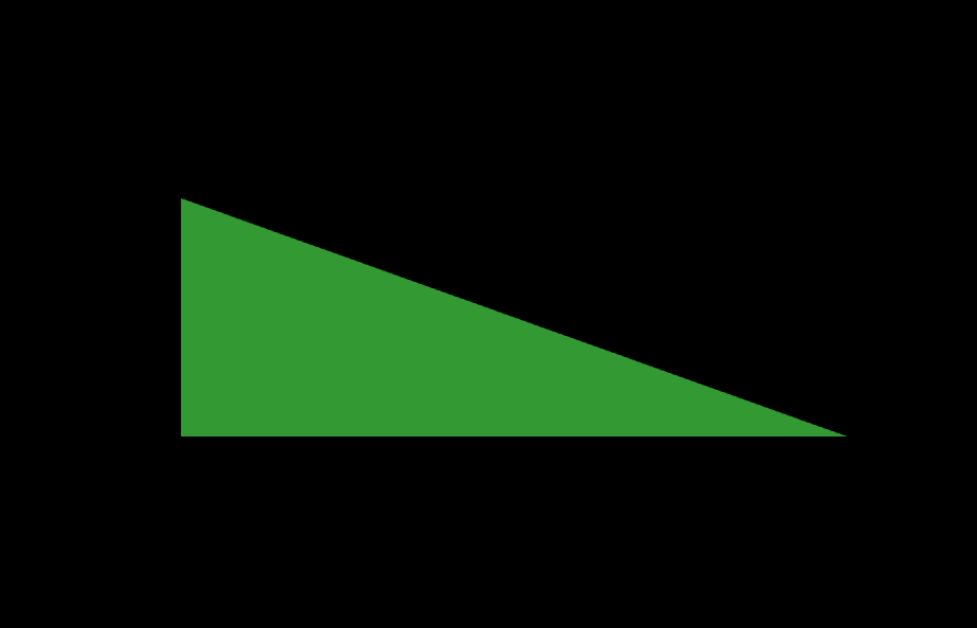
\includegraphics[width=1\columnwidth]{author-files/figures/tri.png}
    \caption{Prototype 1 - A simple 2D triangle drawn using the defined Technology Stack}
    \label{fig:prototype1}
\end{figure}

This was an important milestone in proving the validity of the development process identified. All of the tools and technologies mentioned thus far were setup and used to create a valid WebGL context and render a triangle. It was found that this process was well defined and no changes were done.

\subsubsection {Prototype 2} \label{prototype2}
\begin{figure}[h]
    \centering
    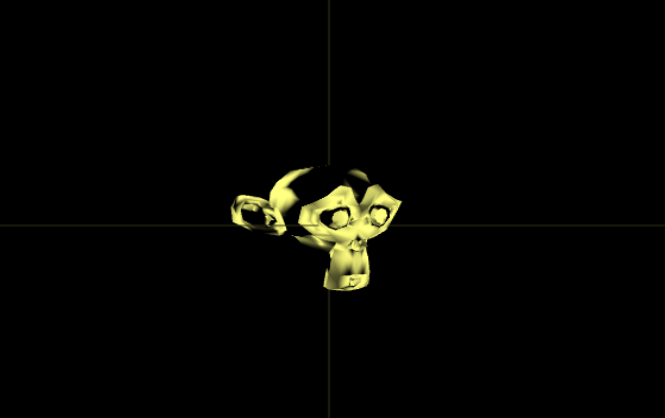
\includegraphics[width=1\columnwidth]{author-files/figures/Monkey-Test2.png}
    \caption{Prototype 2 - A 3D rendering engine}
    \label{fig:Monkey}
\end{figure}

\begin{figure}
    \centering
    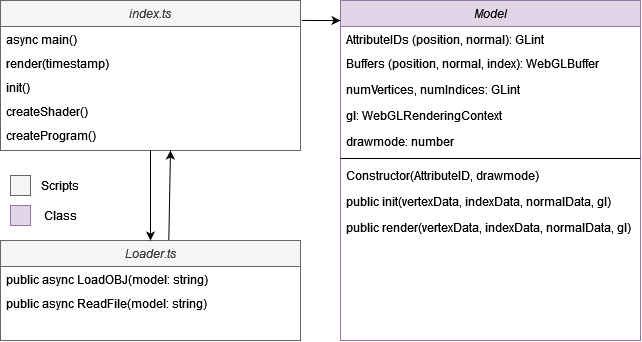
\includegraphics[width=1\columnwidth]{author-files/figures/proto2.png}
    \caption{Prototype 2, Application Class Diagram}
    \label{fig:proto2class}
\end{figure}

\hfill

WebGL is a low level API and considerable work needs to be done just to render a 3D model. With this prototype, the aim was both to further test the tech stacks suitability by doing more involved work, but also to see if a general purpose rendering engine could be created that implemented all of the critical functions for the application to be developed. It was considered important to create this as quickly as possible to identify any shortcomings as soon as possible that may bottleneck the project when development starts. Creating this prototype took approximately a month and yielded in the creation of a successful rendering engine with a charting focused design.

To be more specific, the features implemented by this engine were the following:
\begin{itemize}
    \item 3D Mathematics and View, Projection and model system for rendering
    \item Multiple Models Rendered at the same time
    \item Model Object Abstraction for storing and rendering a 3D model. Implements a prototype pattern where one object can be rendered multiple times. This is particularly useful as a memory saving measure for rendering lot's of models. Something that was considered a very likely scenario for a plotting application with likely many data points.
    \item Simple Flat Shading based on a preset light direction.
    \item Loader Object for loading and organizing data that is passed to Model. Allows .OBJ models to be loaded into the renderer to be displayed.
    \item Rendering labels with HTML and positioning them approximately at some relative to WebGL scene coordinates.
\end{itemize}

Like previously mentioned, This prototype then set the basis from which development was started.

\begin{table*}[t]
    \begin{tabular}{ | l | l | }
        \hline
        Original                                             & Modified                                                    \\
        \hline
        Write chart properties programmatically              & change properties through UI controls                       \\
        \hline
        Static chart image rendered once code written is run & Dynamically update rendered image as properties are changed \\
        \hline
        Difficult to explore                                 & Exploration possible                                        \\
        \hline
    \end{tabular}
    \caption{Comparison of design changes to how figures are created in the application developed compared to programmatic market alternatives}
    \label{}
\end{table*}

\subsection{UX Design} \label{uxdesign}

As mentioned in the research phase- Ease of use and accessibility for non-programmers was a priority for this project. One that had to also dictate design decisions around how a user would interact with the application and how that application would communicate with the user. Those key decisions are mentioned here.

%mention 7 basic tools of quality charts 
\subsubsection{Visualisation Design}
"How should data be plotted and shown to the user?" as a question encapsulates a range of design problems that apply to this section. Specifically, any chart component for this application must embody the following properties to be suitable for completing the application goals:
\begin{itemize}
    \item Must be a common chart type that doesn't require specialist knowledge to understand nor is limited to very specific types of data.
    \item Must be suitable for 3D data and preferably extendable to beyond three dimensions. The more the better.
    \item Chart can be rendered with 3D graphics and preferably that provides some value to the visualizations with the chart type.
\end{itemize}

The chart type that in the end embodied these requirements best was a scatterplot chart. It is a chart that is commonly implemented in 3D by other plotting applications looked at. A scatterplot also naturally fits very well in a 3D rendered environment as it's relatively straight forward to encode plotted data into world coordinates that can be extensively navigated in a 3D environment. Further dimensions can also be encoded by modifying each data point further through colour, saturation, shape of data points, opacity and more.

\begin{figure}[h]
    \centering
    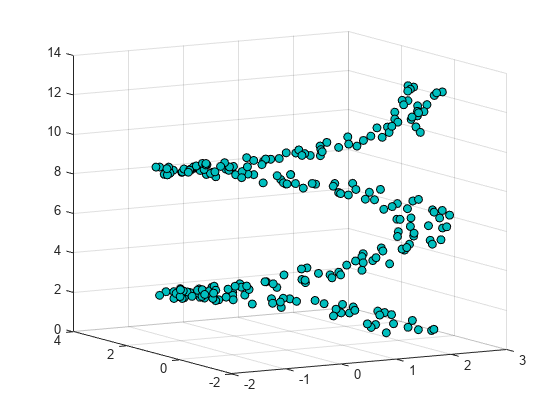
\includegraphics[width=0.7\columnwidth]{author-files/figures/SetMarkerPropertiesExample_01_MATLAB.png}
    \caption{A 3D scatterplot generated through MATLAB, example of a classic cut-off figure}
    \label{fig:MatlabPlot}
\end{figure}

\begin{figure}[h]
    \centering
    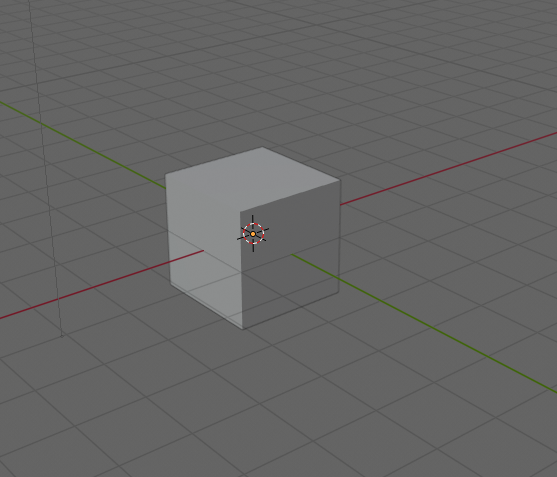
\includegraphics[width=0.7\columnwidth]{author-files/figures/worldnavblender.png}
    \caption{Screenshot from Blender, A 3D modelling application, similar to the Unlimited Axis World view presented}
    \label{fig:MatlabPlot}
\end{figure}

To render the scatterplot, two main ideas were identified.
\begin{itemize}
    \item Unlimited Axis Values, World View. The scatterplot would be rendered into a 3D world by directly translating data values into world coordinates. The resultant graph could then be navigated by the user akin to 3D modelling software or a video game (first-person camera). Axis lines would be part of that world and would extend to infinity from origin. This is a very easy to implement design but might be difficult to navigate for an inexperienced user.
    \item Classic cut-off figure. This is directly inspired by the way the majority of applications seen implement scatterplot. As a user of those systems, you would load in some data and set aspects such as the position, view angle and zoom programmatically which would generate an  image as seen in Figure \ref*{fig:MatlabPlot}. This kind of view is not much harder to render but is much more concise as all data can be made to fit in a predefined visual space. This also allows greater control on how the graph is rendered allowing for a more consistent user experience to be tailored. But, this option has a severe disadvantage- where unlike the previous option, it is not commonly navigated but generated for specific parameters- making exploration not an obvious feature to implement.
\end{itemize}

In the end, the student decided to go with a modified option two. That modification was to replace the programmatic controls that have been seen to be used to compose / generate the chart in applications such as MATLAB with instead similar, although limited UI controls. In a sense, the design that the student came up with abstracts the programming into user controls instead, which are much easier to use (which is the guiding goal for this project) even if they are more limited in their capability.

\subsubsection{User Controls}
The design created by the student in the last section requires a robust design of user controls. With an agile approach, those controls were looked at as the rendering solution improved and opened up possibility for modification.

